\scanpage{49}

et lorsque $i>n$, les \deleted{\unsure{deux}} $H^i(\unsure{\mathfrak g},U(\unsure{m|n}))$ sont nuls d'après b), \inserted{(car $U(\unsure{m|n})$ est fini)}, d'où résulte notre assertion.
\figure{\begin{tikzpicture}\draw (0,0)--(0,.35)--(2.5,.55)..controls (2.7,.55) and (2.8,.6)..(2.8,.75);\end{tikzpicture}}

Si enfin $G$ est \deleted{le groupe} un groupe linéaire unipotent connexe, on distingue deux cas

$1^\circ)$ Caractéristique nulle. Alors $G$ est $\simeq\bar k^n$ sur $\bar k$, donc aussi sur $k$ (en vertu de $H^1(k,\operatorname{Gl}(n))=0$).
Et comme $H^i(k,G_a)=0$ pour $i>0$, l'assertion est valable.

$2^\circ)$ Car. $p\ne0$. Alors on filtre $G$ par $G\supset pG\supset\cdots\supset p^{\unsure{\ell|k}}G=0$. On est ramené au cas où $pG=0$ (les groupes $p^iG$ sont \uline{définis sur $k$}).
\figure{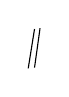
\begin{tikzpicture}\draw (0,0)--(-.08,-.5);\draw (.07,.01)--(0,-.49);\end{tikzpicture}}
Mais, on sait qu'alors $G$ est $\simeq\bar k^{\unsure{n}}$ sur $\bar k$ donc \deleted{$\unsure{\simeq}$} aussi sur $k$ (car $H^1(k,\operatorname{Gl}(n))=0$), et on fait comme dans $1^\circ$.

Supposons que $k$ soit quelconque \ldots

\mspage{48}

